\mode*
\part{Introduction}

\lecture[intro]{intro}{intro}

\section{What's an Operating System}

\begin{frame}{What's an Operating System?}
  \begin{itemize}
  \item \emph{``Everything a vendor ships when you order an operating system''}
  \item It's the program that runs all the time
  \item It's a \alert{resource manager}
    \begin{itemize}
    \item[-] Each program gets time with the resource
    \item[-] Each program gets space on the resource
    \end{itemize}
  \item It's a \alert{control program}
    \begin{itemize}
    \item[-] Controls execution of programs to prevent errors and improper use of the
      computer
    \end{itemize}
  \item No universally accepted definition
  \end{itemize}
\end{frame}

\begin{frame}<beamer>{What's in the OS?}
  \centering \includegraphics[height=.85\textheight]{kernel-block}
\end{frame}

\begin{center}
  \includegraphics[width=.8\textwidth]{kernel-block}
\end{center}

\begin{frame}{Choosing an OS}
  \begin{center}
    \mode<beamer>{ \includegraphics[height=.9\textheight]{choose-os} }%
    \mode<article>{ \includegraphics[width=.6\textwidth]{choose-os} }
  \end{center}
\end{frame}

\begin{frame}{Abstractions}{To hide the complexity of the actual implementations}
  \begin{center}
    \mode<beamer>{ 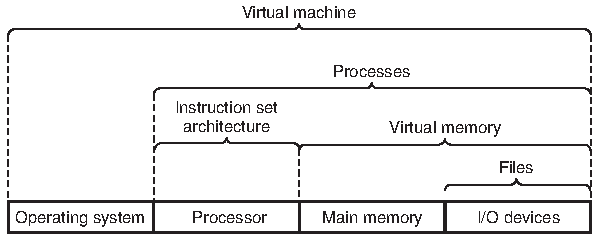
\includegraphics[width=\textwidth]{abstraction} }%
    \mode<article>{ 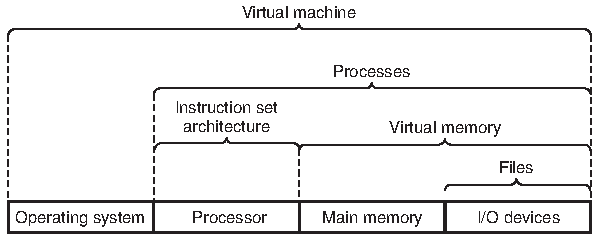
\includegraphics[width=.5\textwidth]{abstraction} }
  \end{center}
\end{frame}

See also: \citetitle[Sec.~1.9.2, \emph{The Importance of Abstractions in Computer
  Systems}]{bryant2010computersystems}.

\begin{frame}{System Goals}
  \begin{block}{Convenient vs. Efficient}
    \begin{itemize}
    \item Convenient for the user --- for PCs
    \item Efficient --- for mainframes, multiusers
    \item UNIX
      \begin{itemize}
      \item[-] Started with keyboard + printer, none paid to convenience
      \item[-] Now, still concentrating on efficiency, with GUI support
      \end{itemize}
    \end{itemize}
  \end{block}
\end{frame}

\begin{frame}{History of Operating Systems}
  \begin{center}
    \mode<beamer>{ 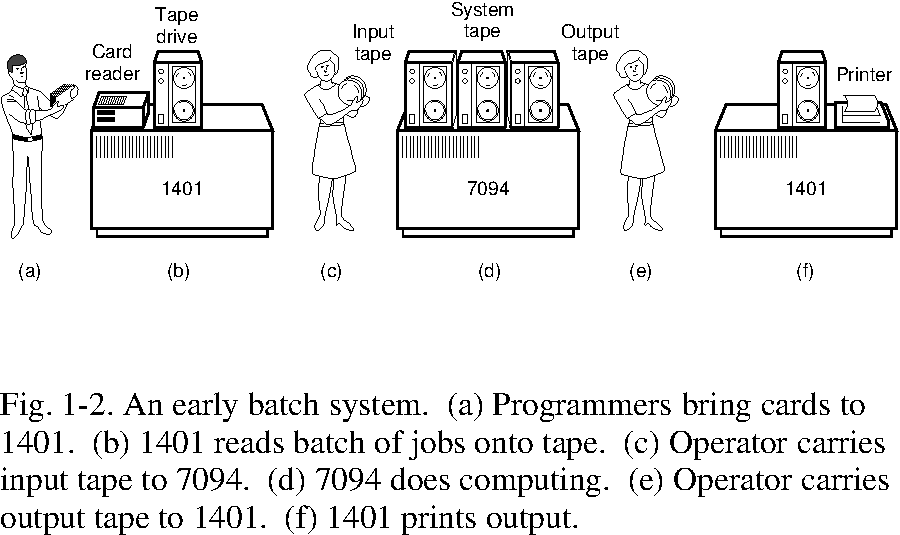
\includegraphics[height=.9\textheight]{mos-figs-1-2} }%
    \mode<article>{ 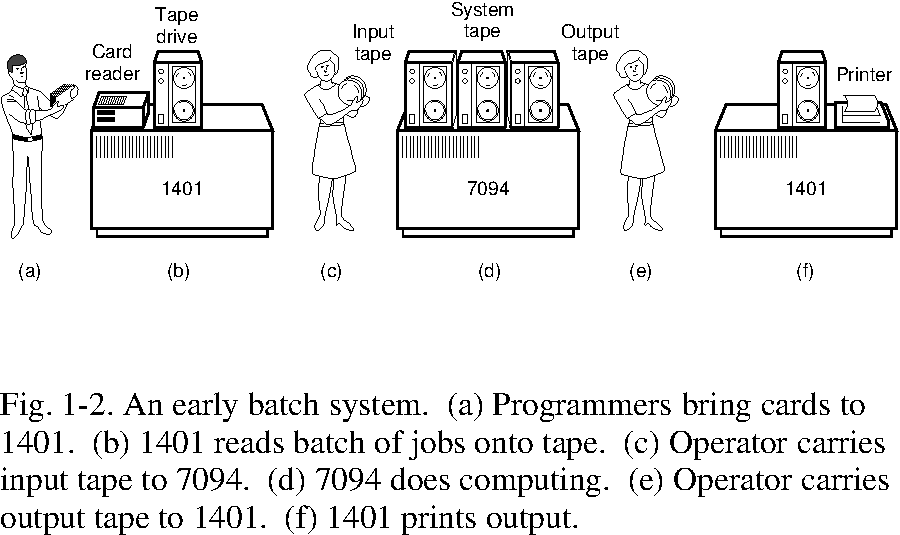
\includegraphics[width=.7\textwidth]{mos-figs-1-2} }
  \end{center}
\end{frame}

\begin{frame}
  \begin{minipage}{.4\linewidth}
    \begin{description}
    \item[1945 -- 1955] 1\textsuperscript{st} generation
    \item[] vacuum tubes, plug boards
    \item[1955 -- 1965] 2\textsuperscript{nd} generation
    \item[] transistors, batch systems
    \item[1965 -- 1980] 3\textsuperscript{rd} generation
    \item[] ICs and multiprogramming
    \item[1980 -- present] 4\textsuperscript{th} generation
    \item[] personal computers
    \end{description}
  \end{minipage}\;
  \begin{minipage}{.55\linewidth}
    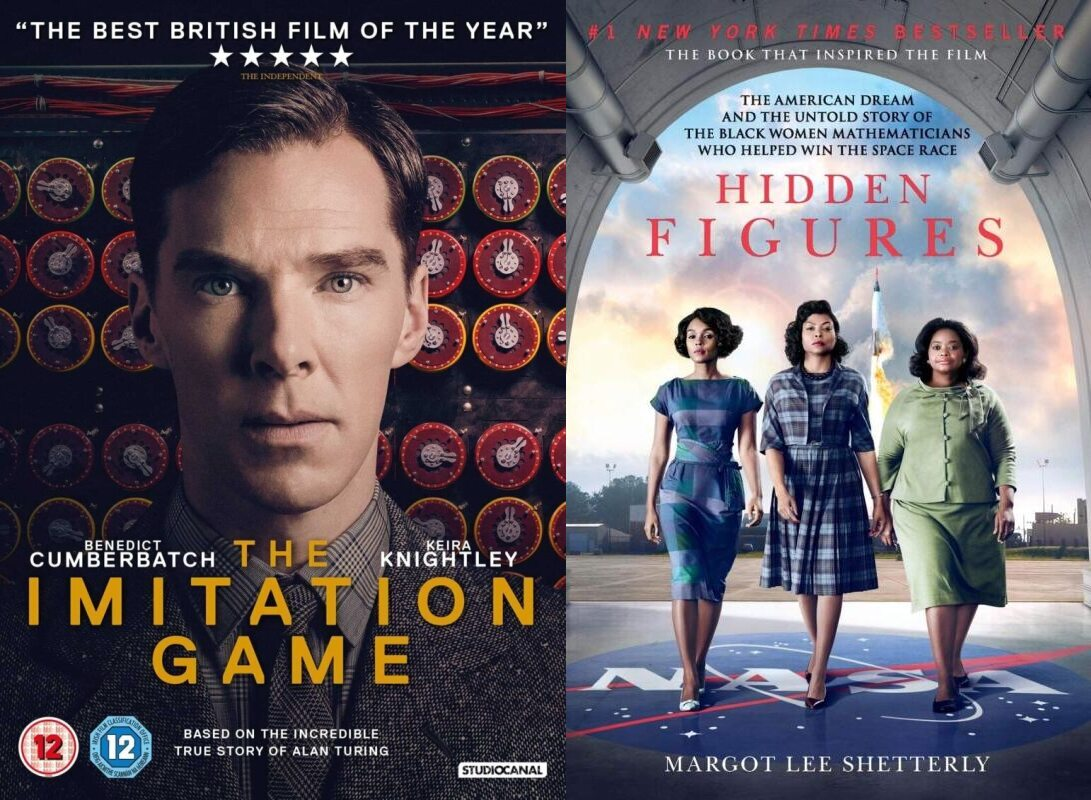
\includegraphics[width=1.1\textwidth]{movies}
  \end{minipage}
  \end{frame}

\begin{frame}
  \begin{block}{Multi-programming is the first instance where the OS must make decisions
      for the users}
    \begin{minipage}{.65\linewidth}
      \begin{description}
      \item[Job scheduling] --- decides which job should be loaded into the memory.
      \item[Memory management] --- because several programs in memory at the same time
      \item[CPU scheduling] --- choose one job among all the jobs are ready to run
      \item[Process management] --- make sure processes don't offend each other
      \end{description}
    \end{minipage}\quad
    \begin{minipage}{.3\linewidth}
      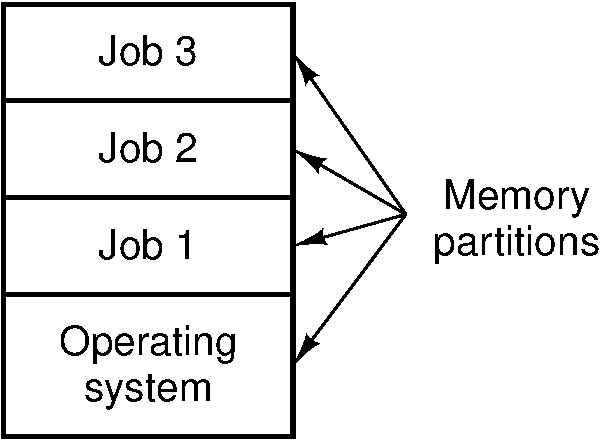
\includegraphics[width=\textwidth]{mos-figs-1-4}
    \end{minipage}
  \end{block}
\end{frame}

\begin{frame}{The Operating System Zoo}
  \begin{minipage}{.45\linewidth}
    \begin{itemize}
    \item {\huge Mainframe OS}
    \item {\LARGE Server OS}
    \item {\Large Multiprocessor OS}
    \item {\large Personal computer OS}
    \item Real-time OS
    \item {\small Embedded OS}
    \item {\scriptsize Smart card OS}
    \end{itemize}
  \end{minipage}\quad
  \begin{minipage}{.45\linewidth}
    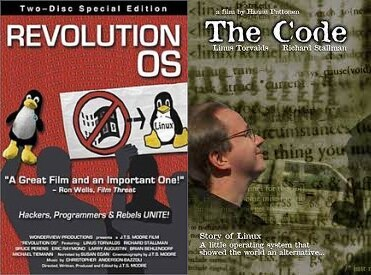
\includegraphics[width=\textwidth]{movies2}
  \end{minipage}
\end{frame}

\section{OS Services}

\begin{frame}{OS Services}{Like a government}
  \begin{block}{Helping the users:}
    \begin{multicols}{2}
      \begin{itemize}
      \item User interface
      \item Program execution
      \item I/O operation
      \item File system manipulation
      \item Communication
      \item Error detection
      \end{itemize}
    \end{multicols}
  \end{block}
  \begin{minipage}{.4\linewidth}
    \begin{block}{Keeping the system efficient:}
      \begin{itemize}
      \item Resource allocation
      \item Accounting
      \item Protection and security
      \end{itemize}
    \end{block}
  \end{minipage}\qquad
  \begin{minipage}{.5\linewidth}
    \begin{tblr}{colspec={cX[c,3em]c},hline{2,3}={1,3}{solid}}
      User processes&&People\\
      OS&vs.&Government\\
      Hardware&&Country\\
    \end{tblr}
    % \begin{iblock}{}
    %   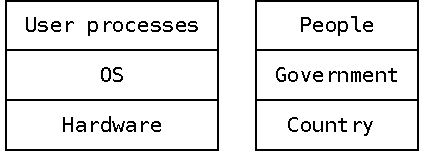
\includegraphics[width=\textwidth]{os-gov}
    % \end{iblock}
  \end{minipage}
\end{frame}

\begin{frame}{A Computer System}
  \begin{center}
    \mode<beamer>{ 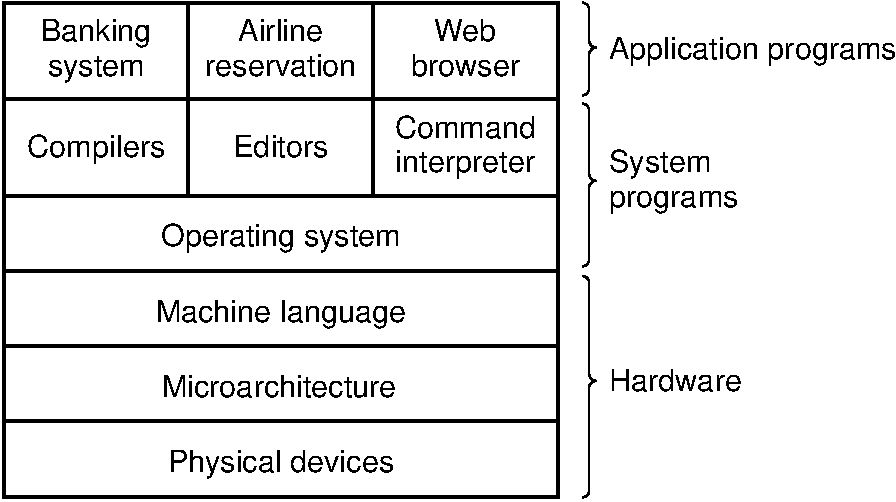
\includegraphics[width=.8\textwidth]{mos-figs-1-1} }%
    \mode<article>{ 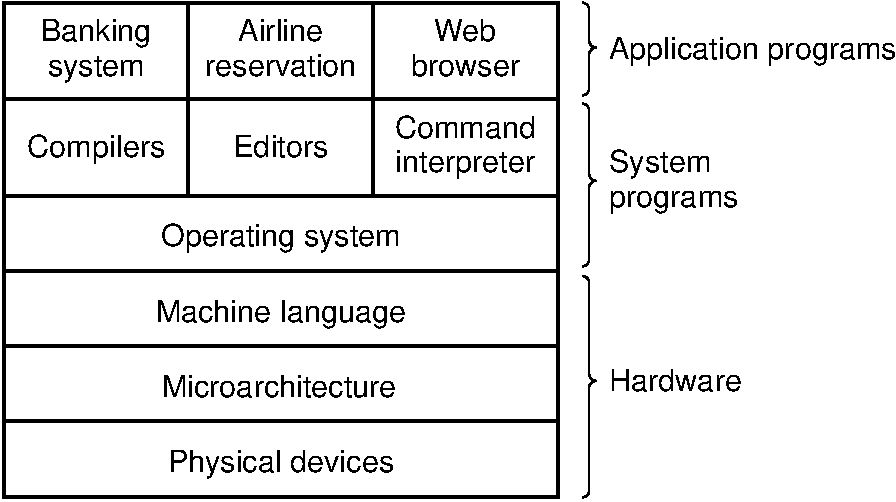
\includegraphics[width=.5\textwidth]{mos-figs-1-1} }
  \end{center}
\end{frame}

\begin{frame}{HarmonyOS}
  \begin{tikzpicture}[remember picture,overlay]
    \node[anchor=south,yshift=3mm,inner sep=0pt] at (current page.south) {
      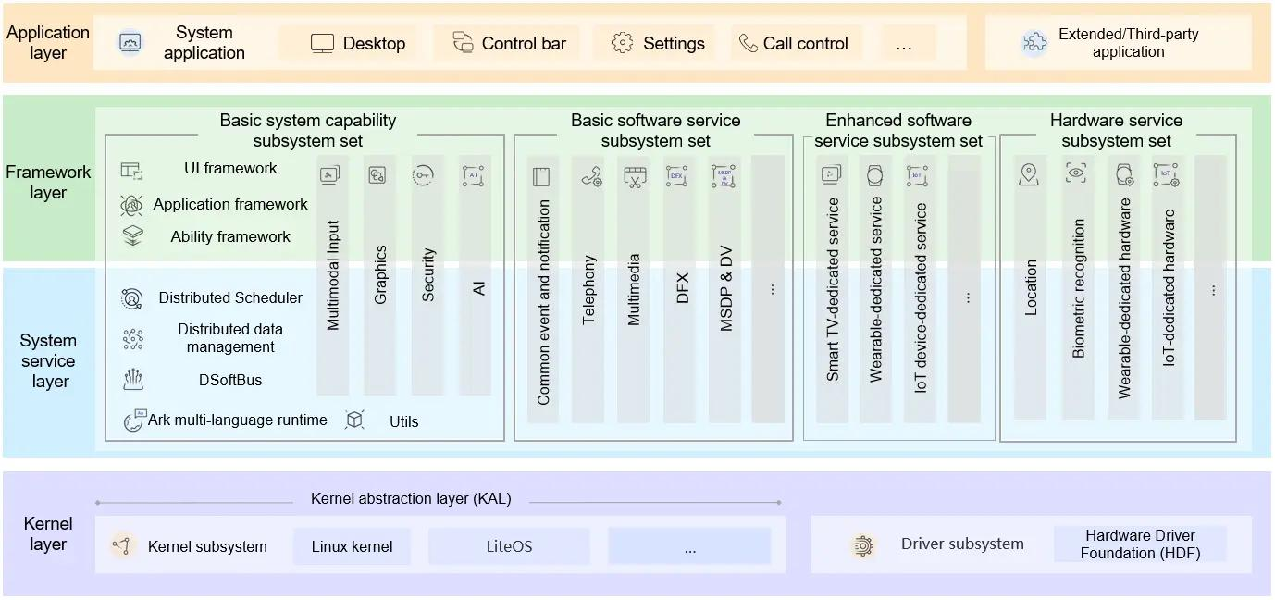
\includegraphics[width=\paperwidth]{HarmonyOS} };
  \end{tikzpicture}
\end{frame}

\section{Hardware}
\label{sec:cpu}

% \begin{frame}<beamer>{Outline}
%   \tableofcontents[currentsection,currentsubsection]
% \end{frame}

\begin{frame}{CPU Working Cycle}
  \begin{center}
    \begin{tblr}{colspec={ccccc},vlines,hlines={1-1,3-3,5-5}{},row{1}={m}}
      {Fetch\\{}unit}&➠&{Decode\\{}unit}&➠&{Execute\\{}unit}
    \end{tblr}
    % \mode<beamer>{ 
\includegraphics[width=.6\textwidth]{mos-figs-1-6} }%
    % \mode<article>{ 
\includegraphics[width=.3\textwidth]{mos-figs-1-6} }
  \end{center}
  \begin{enumerate}
  \item Fetch the first instruction from memory
  \item Decode it to determine its type and operands
  \item Execute it
  \end{enumerate}
  \begin{block}{Special CPU Registers}
    \begin{description}
    \item[Program counter (PC):] keeps the memory address of the next instruction to
      be fetched
    \item[Stack pointer (SP):] {\symbola ☛} the top of the current stack in memory
    \item[Program status (PS):] holds
      \begin{itemize}
      \item[-] condition code bits
      \item[-] processor state
      \end{itemize}
    \end{description}
  \end{block}
\end{frame}

\begin{frame}{System Bus}
  \begin{center}
    \mode<beamer>{ 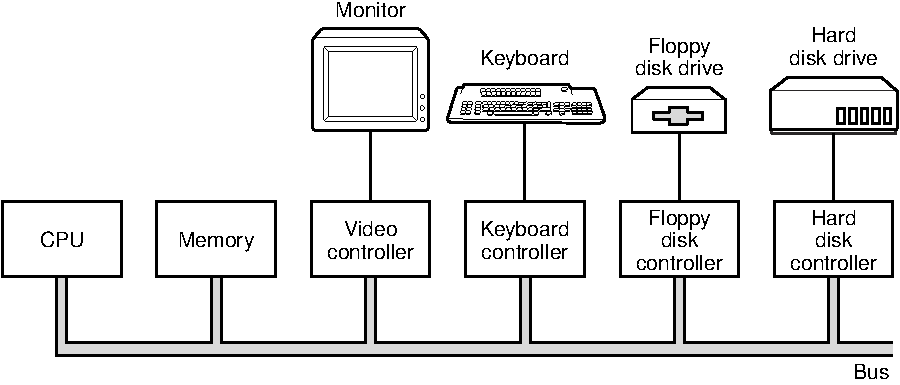
\includegraphics[width=.8\textwidth]{mos-figs-1-5} }%
    \mode<article>{ 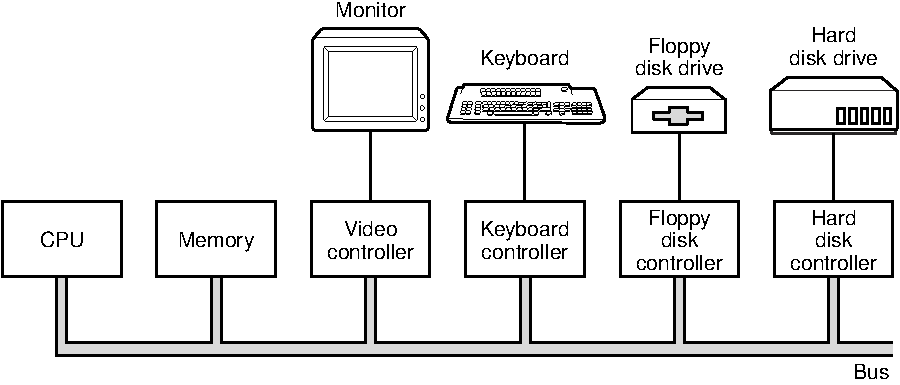
\includegraphics[width=.6\textwidth]{mos-figs-1-5} }
  \end{center}
  \begin{description}
  \item[Address Bus:] specifies the memory locations (addresses) for the
    data transfers
  \item[Data Bus:] holds the data transfered. Bidirectional
  \item[Control Bus:] contains various lines used to route timing and
    control signals throughout the system
  \end{description}
\end{frame}

\begin{frame}{Controllers and Peripherals}
  \begin{itemize}
  \item Peripherals are real devices controlled by controller chips
  \item Controllers are processors like the CPU itself, have control registers
  \item Device driver writes to the registers, thus control it
  \item Controllers are connected to the CPU and to each other by a variety of buses
  \end{itemize}
\end{frame}

\begin{frame}[label=current]
  \begin{center}
    \mode<beamer>{ 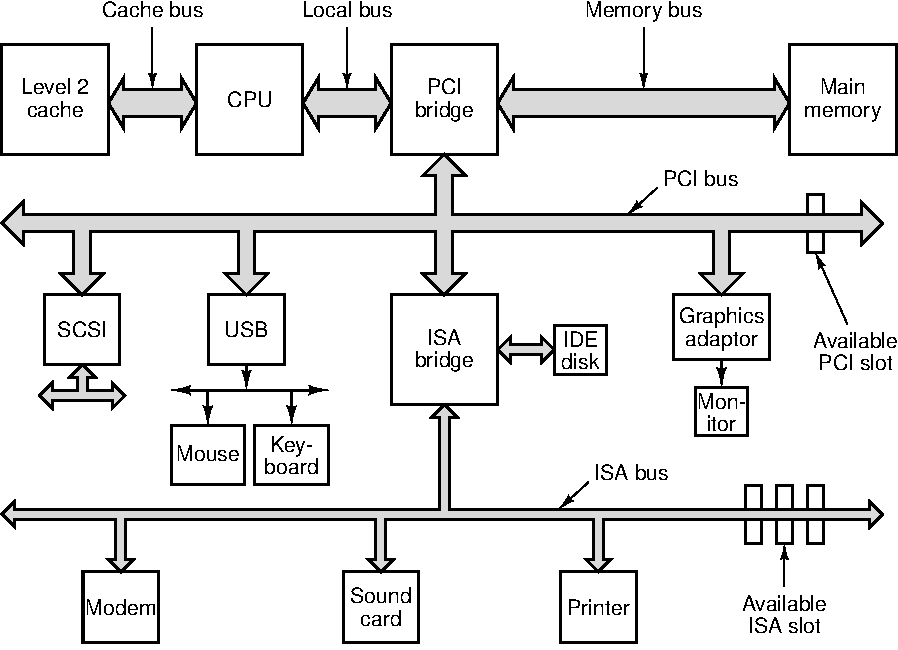
\includegraphics[height=.9\textheight]{mos-figs-1-11} }%
    \mode<article>{ 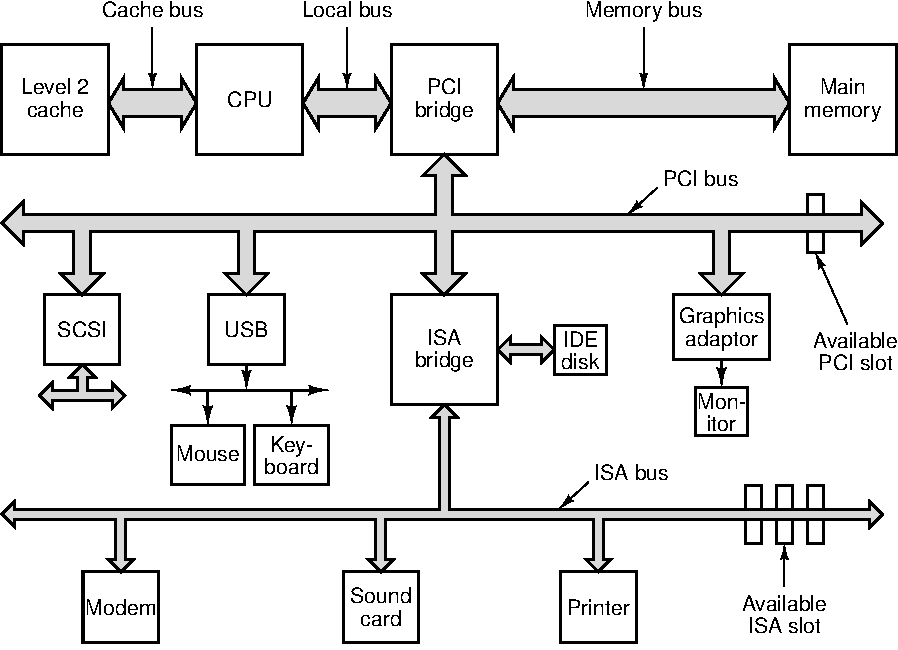
\includegraphics[width=.6\textwidth]{mos-figs-1-11} }
  \end{center}
\end{frame}

\begin{frame}{Motherboard Chipsets}
  \begin{center}
    \mode<beamer>{ 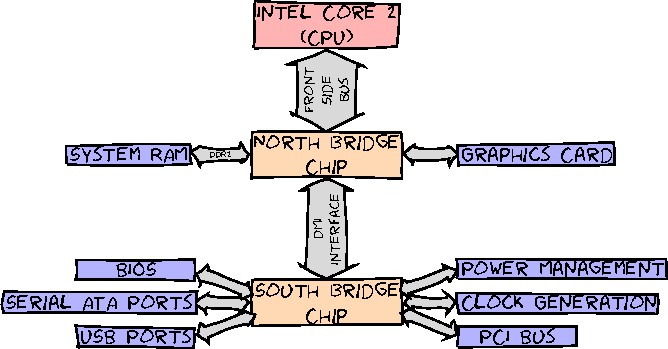
\includegraphics[width=.6\textwidth]{chipsets} }
    \mode<article>{ \includegraphics[width=.5\textwidth]{chipsets-bw} }
  \end{center}
  \begin{block}{The northbridge}
    \begin{enumerate}
    \item receives a physical memory request
    \item decides where to route it
      \begin{itemize}
      \item[-] to RAM? to video card? to \ldots{}?
      \item[-] decision made via the \alert{memory address map}
      \end{itemize}
    \end{enumerate}
  \end{block}
\end{frame}

See also:
\begin{itemize}
\item When is the memory address map built? \texttt{setup()}.
\item
  \href{http://duartes.org/gustavo/blog/post/motherboard-chipsets-memory-map}{\emph{Motherboard
      Chipsets And The Memory Map}}
  \footnote{\url{http://duartes.org/gustavo/blog/post/motherboard-chipsets-memory-map}}.
\end{itemize}


\begin{frame}
  \begin{itemize}
  \item The CPU doesn't know what it's connected to
    \begin{itemize}
    \item[-] CPU test bench?\quad{}network router?\quad{}toaster?\quad{}brain implant?
    \end{itemize}
  \item The CPU talks to the outside world through its pins
    \begin{itemize}
    \item[-] some pins to transmit the physical memory address
    \item[-] other pins to transmit the values
    \end{itemize}
  \item The CPU's gateway to the world is the \alert{front-side bus}
  \end{itemize}
  \begin{block}{Intel Core 2 QX6600}
    \begin{itemize}
    \item 33 pins to transmit the physical memory address
      \begin{itemize}
      \item[-] so there are \(2^{33}\) choices of memory locations
      \end{itemize}
    \item 64 pins to send or receive data
      \begin{itemize}
      \item[-] so data path is 64-bit wide, or 8-byte chunks
      \end{itemize}
    \end{itemize}
    This allows the CPU to physically address \unit[64]{GiB} of memory (\(2^{33}\times{}8\,B\))
  \end{block}
\end{frame}

See also:
\href{http://download.intel.com/design/processor/datashts/31559205.pdf}{\emph{Datasheet
    for Intel Core 2 Quad-Core Q6000 Sequence}}
\footnote{\url{http://download.intel.com/design/processor/datashts/31559205.pdf}}.

\begin{frame}[plain]
  \begin{minipage}{.55\linewidth}
    \begin{block}{Some physical memory addresses are mapped away!}
      \begin{itemize}
      \item only the addresses, not the spaces
      \item Memory holes
        \begin{itemize}
        \item[-] \unit[640]{KiB}~\char`~~\unit[1]{MiB}
        \item[-] \texttt{/proc/iomem}
        \end{itemize}
      \end{itemize}
    \end{block}
    \begin{block}{Memory-mapped I/O}
      \begin{itemize}
      \item BIOS ROM
      \item video cards
      \item PCI cards
      \item \ldots
      \end{itemize}
      This is why 32-bit OSes have problems using \unit[4]{GiB} of RAM.
    \end{block}
  \end{minipage}\quad
  \begin{minipage}{.35\linewidth}
    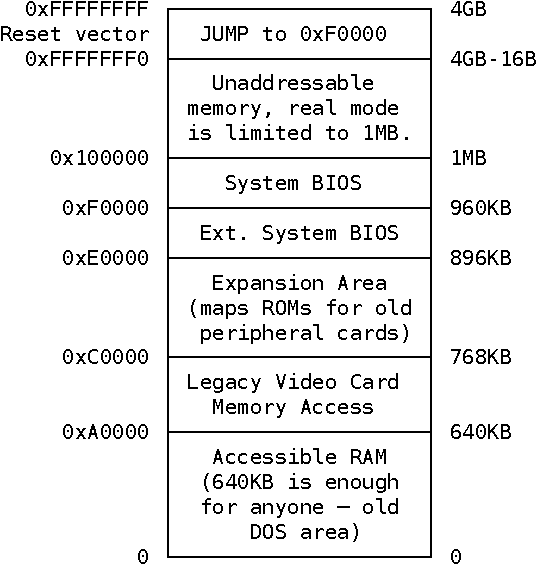
\includegraphics[scale=.7]{boot-mem}
  \end{minipage}
\end{frame}

\section{Bootstrapping}
\label{sec:bootstrapping}

\begin{frame}{Bootstrapping}
  \begin{minipage}{.85\linewidth}
    \begin{block}{Can you pull yourself up by your own bootstraps?}
      A computer cannot run without first loading software but must be
      running before any software can be loaded.
    \end{block}
  \end{minipage}\hfill
  \begin{minipage}{.1\linewidth}
    \includegraphics[width=\textwidth]{bootstrap}
  \end{minipage}
    \begin{center}
    \mode<beamer>{ 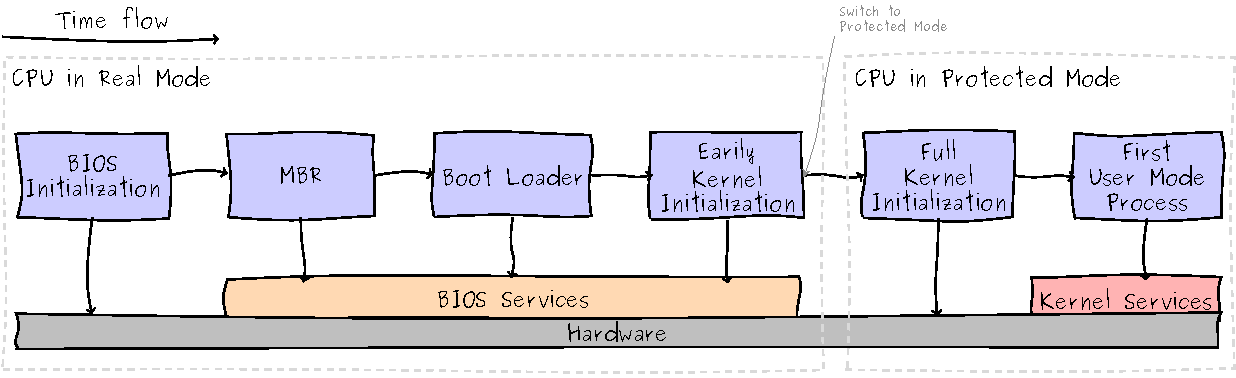
\includegraphics[width=\textwidth]{boot}}%
    \mode<article>{ \includegraphics[width=.7\textwidth]{boot-bw}}
  \end{center}
\end{frame}

\begin{frame}{Intel x86 Bootstrapping}
  \begin{enumerate}
  \item BIOS (\texttt{0xfffffff0})\\
    \begin{small}
      ➠ POST\quad
      ➠ HW init\quad
      ➠ Find a boot device (FD, CD, HD\ldots{})\quad
      ➠ Copy \alert{sector zero (MBR)} to RAM (\texttt{0x00007c00})
    \end{small}
  \item MBR -- the first \unit[512]{Bytes}, contains
    \begin{itemize}
    \item Small code (⩽ \unit[446]{Bytes}), e.g. GRUB stage 1, for loading GRUB stage 2
    \item the primary partition table ($16\times{}4=64\,Bytes$)
    \end{itemize}
    Its job is to load the 2\textsuperscript{nd} stage boot loader.
  \item GRUB stage 2 --- load the OS kernel into RAM
  \item {} startup
  \item init --- the first user-space program
  \end{enumerate}
  \begin{center}
    \mode<beamer>{ \includegraphics[width=.8\textwidth]{mbr}}%
    \mode<article>{ \includegraphics[width=.5\textwidth]{mbr}}
  \end{center}
  \CMD{sudo hd -n512 /dev/sda}
\end{frame}

\begin{frame}{Inter-compatible Processors Are Little-endian}
  \begin{iblock}{To store \texttt{0x01234567} into memory}
    \begin{center}
      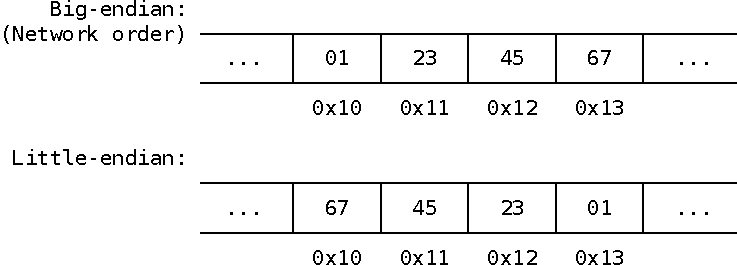
\includegraphics[width=.7\textwidth]{0xaa55}
    \end{center}
  \end{iblock}
\end{frame}

\section{Interrupt}
\label{sec:interrupt}

% \begin{frame}<beamer>{Outline}
%   \tableofcontents[currentsection,currentsubsection]
% \end{frame}

\begin{frame}{Why Interrupt?}
  \begin{iblock}{While a process is reading a disk file, can we do\ldots}
    \begin{center}
      \mode<beamer>{ \includegraphics[width=.6\textwidth]{interrupt-c}}%
      \mode<article>{ \cfile{./figs/pseudo/interrupt.c}}
    \end{center}
  \end{iblock}
\end{frame}

\begin{frame}{Modern OS are Interrupt Driven}
  \begin{description}
  \item[HW INT] by sending a signal to CPU
  \item[SW INT] by executing a \alert{system call}
  \item[Trap (exception)] is a software-generated INT coursed by an error or by a
    specific request from an user program
  \item[Interrupt vector] is an array of pointers ☛ the memory addresses
    of \alert{interrupt handlers}. This array is indexed by a unique device number
    \begin{itemize}
    \item[] \CMD{less /proc/devices}
    \item[] \CMD{less /proc/interrupts}
    \end{itemize}
  \end{description}
\end{frame}

\begin{frame}{Programmable Interrupt Controllers}
  \begin{center}
    \mode<beamer>{ 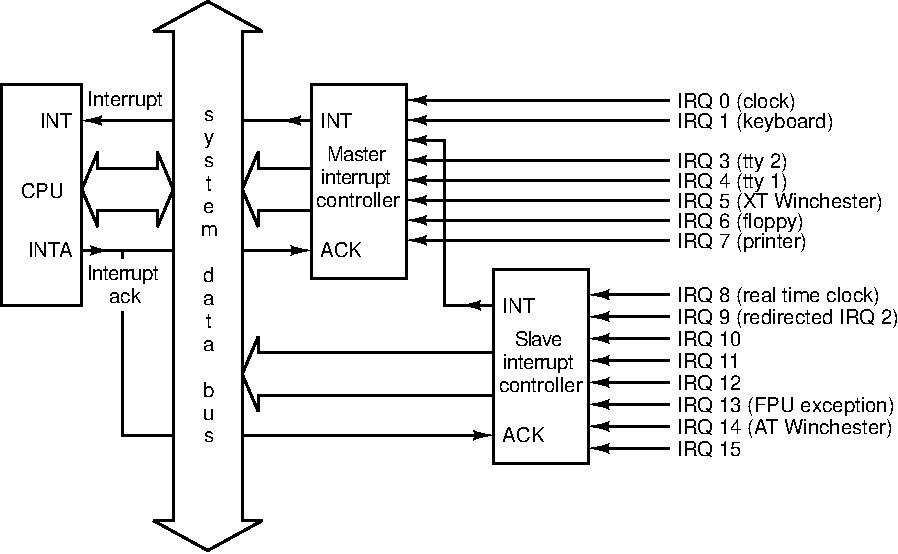
\includegraphics[height=.9\textheight]{int-osdi-34}}%
    \mode<article>{ 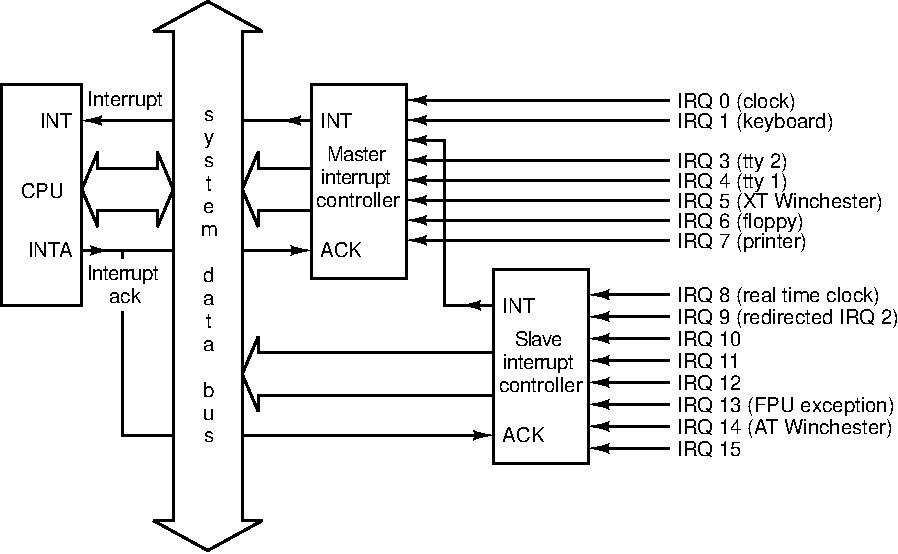
\includegraphics[width=.5\textwidth]{int-osdi-34}}
  \end{center}
\end{frame}

\begin{frame}{Interrupt Processing}
  % 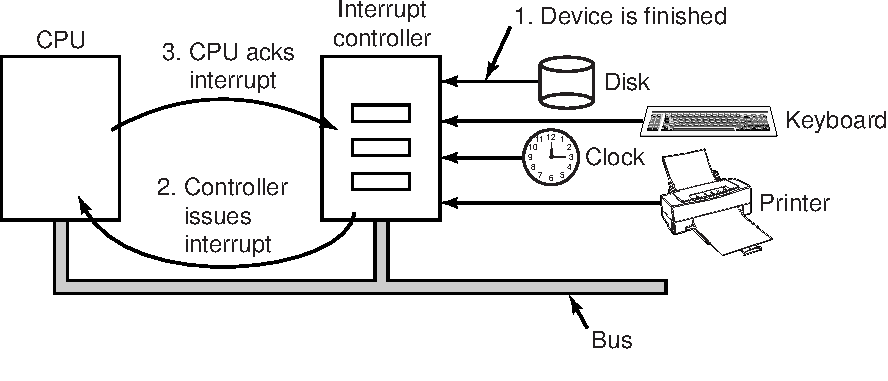
\includegraphics[width=.9\textwidth]{int-mos-figs-5-6}\\
  \begin{center}
    \mode<beamer>{ 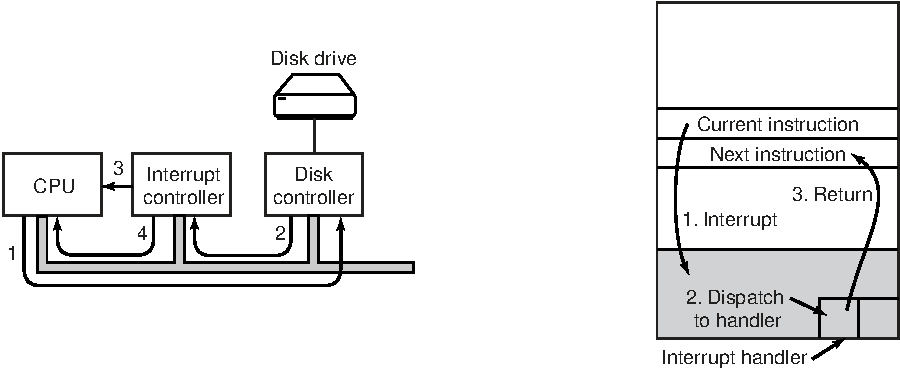
\includegraphics[width=\textwidth]{mos-figs-1-10} }%
    \mode<article>{ 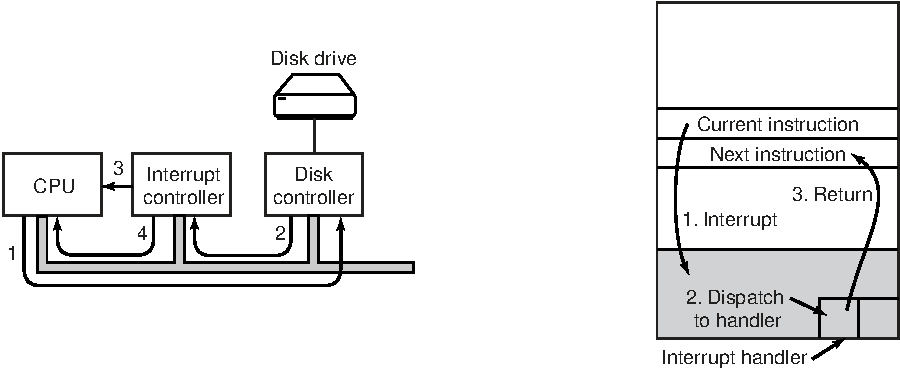
\includegraphics[width=.7\textwidth]{mos-figs-1-10} }
  \end{center}
\end{frame}

Detailed explanation: in \citetitle[Sec.~1.3.5, \emph{I/O Devices}]{tanenbaum2015modern}.

\begin{frame}{Interrupt Timeline}
  \begin{center}
    \mode<beamer>{ 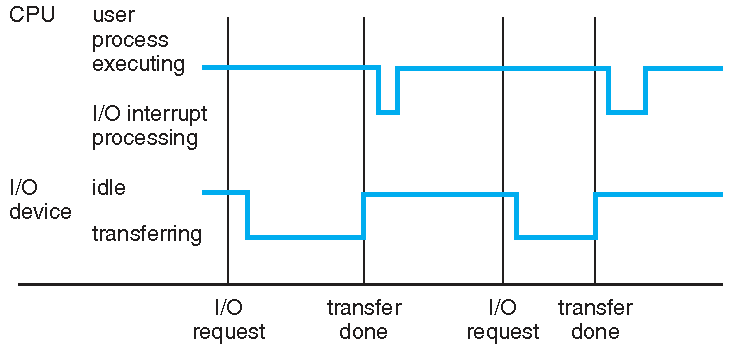
\includegraphics[width=\textwidth]{ir-timeline} }%
    \mode<article>{ 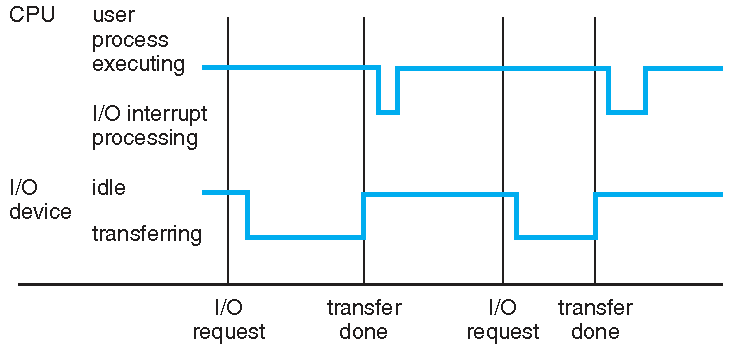
\includegraphics[width=.5\textwidth]{ir-timeline} }
  \end{center}
\end{frame}

\section{System Calls}
\label{sec:system-calls}

% \begin{frame}<beamer>{Outline}
%   \tableofcontents[currentsection,currentsubsection]
% \end{frame}

\begin{frame}{System Calls}
  \begin{block}{A System Call}
    \begin{itemize}
    \item is how a program requests a service from an OS kernel
    \item provides the interface between a process and the OS
    \end{itemize}
  \end{block}
  \begin{itemize}
  \item[] \CMD{man 2 intro}
  \item[] \CMD{man 2 syscalls}
  \end{itemize}
\end{frame}

\begin{frame}<beamer>
  \centering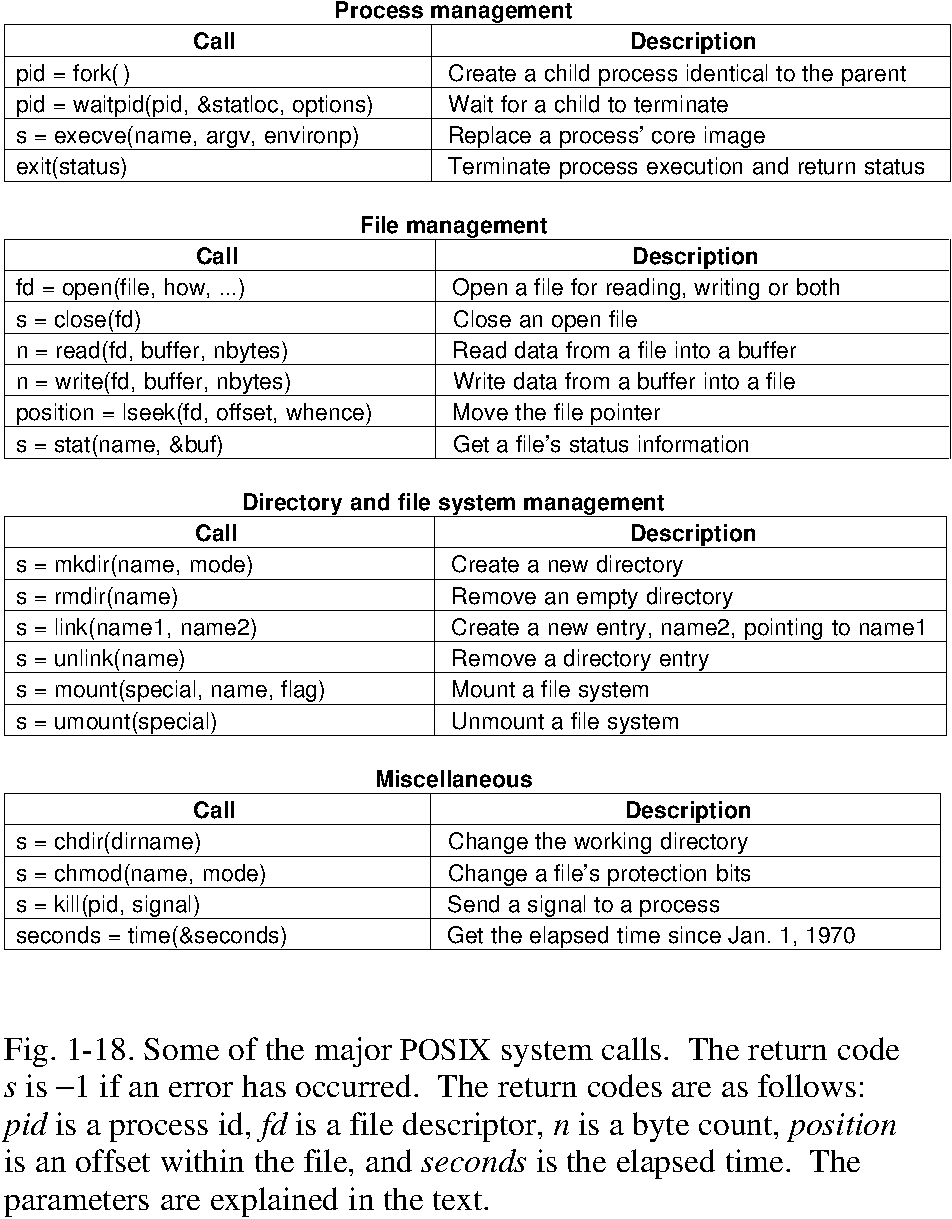
\includegraphics[width=.6\textwidth]{mos-figs-1-19}
\end{frame}

\begin{center}
  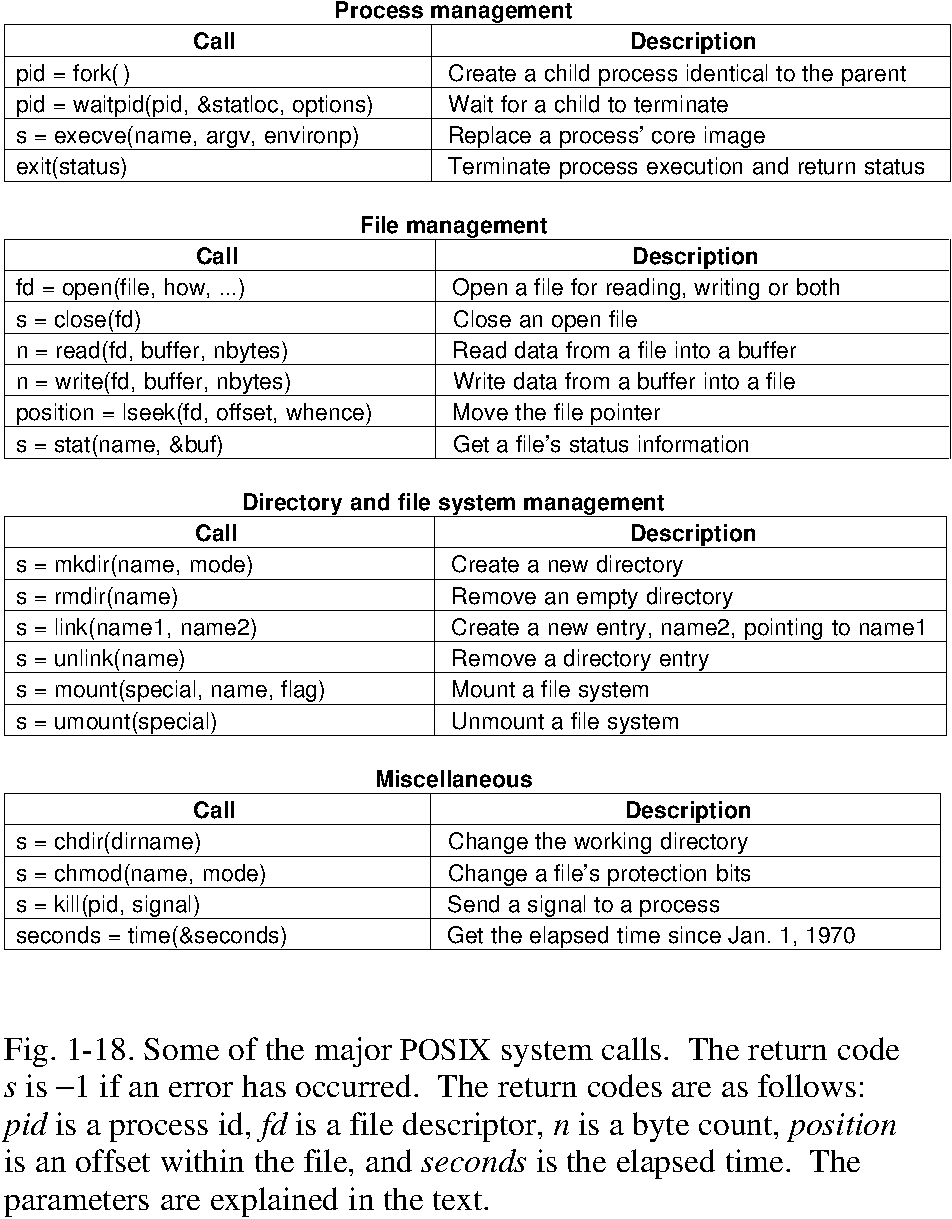
\includegraphics[width=.7\textwidth]{mos-figs-1-19}
\end{center}

\begin{frame}<beamer>
  \centering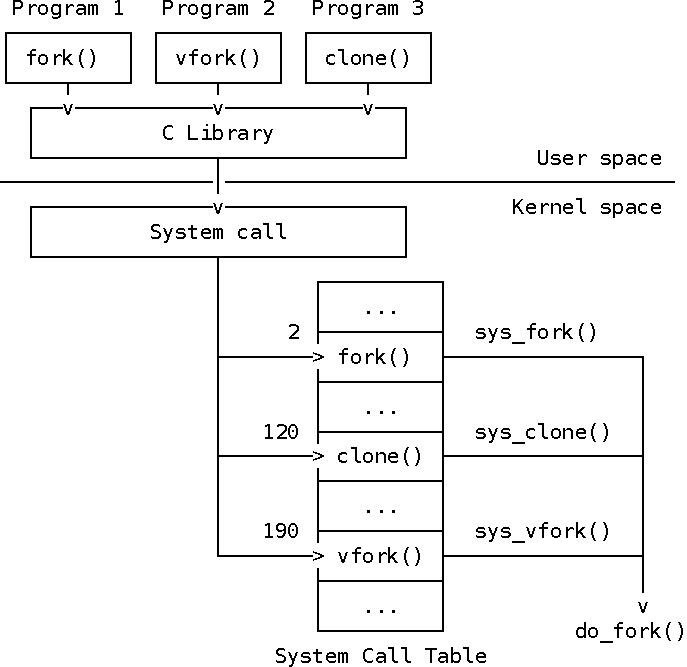
\includegraphics[height=\textheight]{syscall}
\end{frame}

\begin{frame}<beamer>
  \centering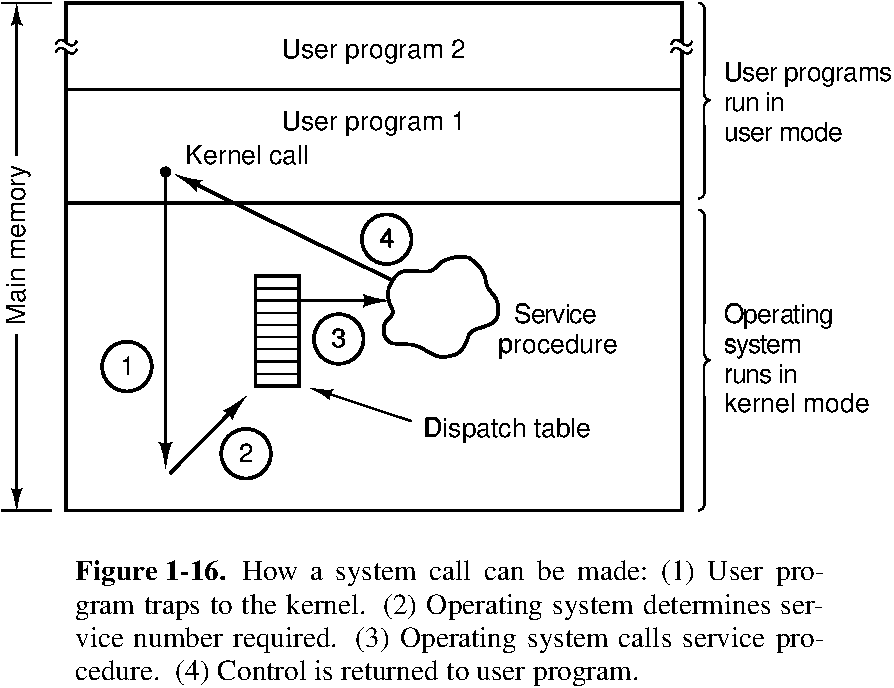
\includegraphics[height=.9\textheight]{osdi2-1-18}
\end{frame}

\begin{center}
  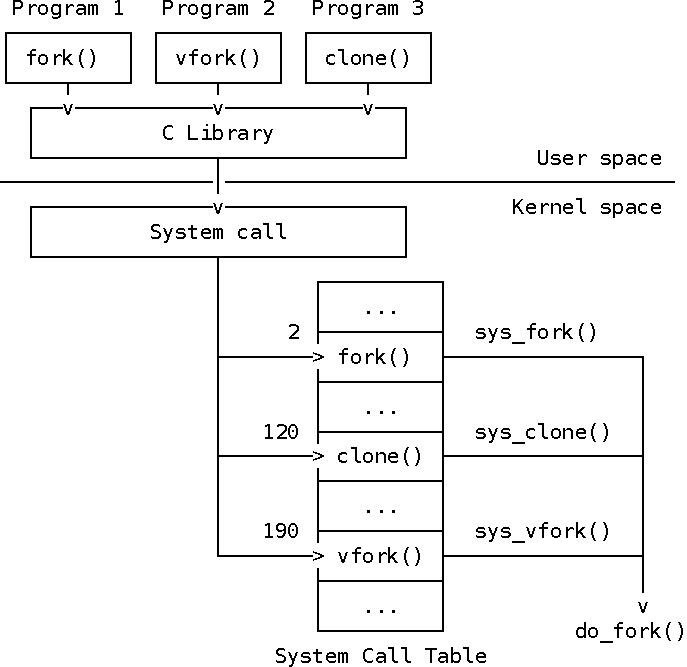
\includegraphics[width=.45\textwidth]{syscall}\quad
  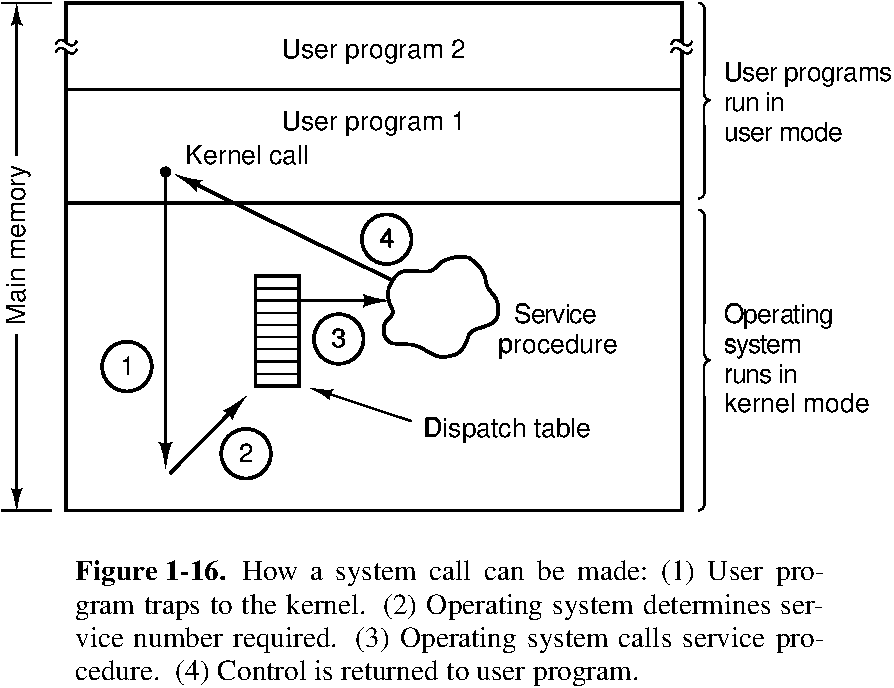
\includegraphics[width=.5\textwidth]{osdi2-1-18}
\end{center}

% \begin{frame} {System Calls}
%   \includegraphics[width=\textwidth]{syscall1}
% \end{frame}

\begin{frame}<beamer>{\texttt{read(fd, buffer, nbytes)}}
  \begin{minipage}{.3\linewidth}
    \CMD{man 2 read}
  \end{minipage}\quad
  \begin{minipage}{.65\linewidth}
    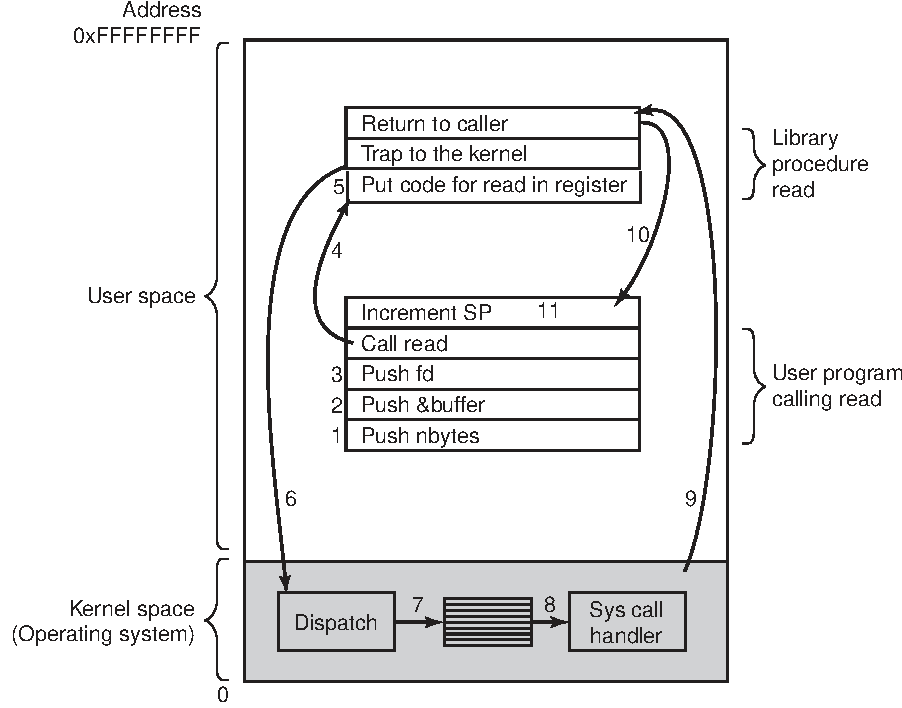
\includegraphics[width=\textwidth]{mos-figs-1-18}
  \end{minipage}
\end{frame}

\begin{center}
  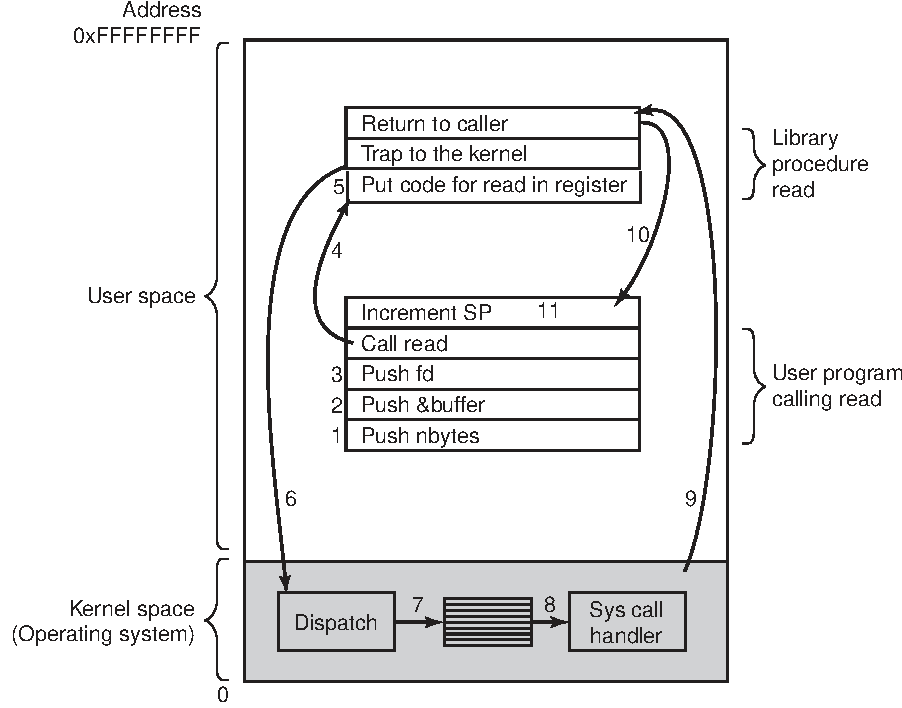
\includegraphics[width=.7\textwidth]{mos-figs-1-18}
  \captionof{figure}{The 11 steps to make syscall \texttt{read(fd, buffer, nbytes)}}
\end{center}  

\begin{frame}{Example}{Linux INT80h}
  \begin{description}
  \item[Interrupt Vector Table:] The very first \unit[1]{KiB} of x86 memory. 
    \begin{itemize} 
    \item 256 entries $\times$ \unit[4]{B} = \unit[1]{KiB}
    \item Each entry is a complete memory address (segment:offset)
    \item It's populated by Linux and BIOS
    \item Slot 80h: address of the kernel services dispatcher (☛ sys-call table)
    \end{itemize}
  \end{description}
\end{frame}

\begin{itemize}
\item \url{https://github.com/torvalds/linux/blob/master/arch/x86/entry/syscalls/syscall_64.tbl}
\end{itemize}

\begin{frame}{Example}
  \begin{center}
    \mode<beamer>{ 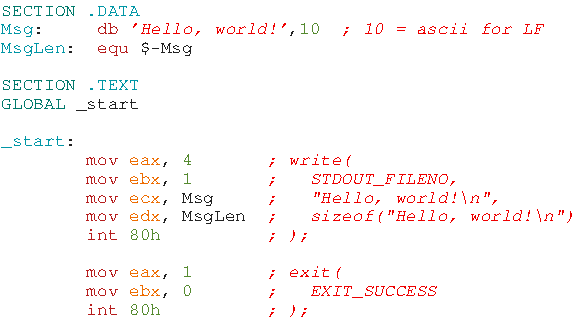
\includegraphics[width=.8\textwidth]{hello32-asm} }%h-asm.pdf
    \mode<article>{ \nasmfile{../src/hello-nasm/hello32.asm}}
  \end{center}
%  System call numbers:
  \begin{itemize}
  \item[] \CMD{less /usr/include/x86\_64-linux-gnu/asm/unistd\_32.h}
  \item[] \CMD{less /usr/include/x86\_64-linux-gnu/asm/unistd\_64.h}
  \end{itemize}
\end{frame}

64-bits version:
\nasmfile{../src/hello-nasm/hello64.s}

\begin{frame}{System Call Examples}
  \begin{minipage}{.55\linewidth}
    \mode<beamer>{ \includegraphics[width=\textwidth]{write-c} }%
    \mode<article>{ \cfile{../src/fs/write.c}}
  \end{minipage}\quad
  \begin{minipage}{.4\linewidth}\ttfamily\footnotesize
    \begin{itemize}
    \item Actually, \texttt{write()} is a wrapper function in glibc.
    \item[] \CMD{man 2 write}
    \item[] \CMD{man 3 write}
    \end{itemize}
  \end{minipage}\\[1em]
  \begin{description}
  \item[Don't invoke syscall directly whenever possible]
  \end{description}
  \mode<beamer>{ \centering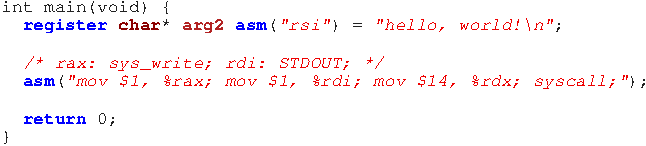
\includegraphics[width=.9\textwidth]{write-inlineasm-c} }%
  \mode<article>{ \cfile{../src/fs/write-inlineasm.c}}
\end{frame}

\begin{itemize}
\item \url{https://jameshfisher.com/2018/02/20/c-inline-assembly-hello-world/}
\item \url{https://cs.lmu.edu/~ray/notes/gasexamples/}
\item \url{https://montcs.bloomu.edu/Information/LowLevel/Assembly/assembly-tutorial.html}
\end{itemize}

\begin{frame}{System Call Examples}
  \CMD{man 2 fork}
  \begin{center}
    \mode<beamer>{ \includegraphics[width=.6\textwidth]{fork-c} }%
    \mode<article>{ \cfile{../src/proc/fork.c}}
  \end{center}
\end{frame}

\begin{frame}
  \CMD{man 3 exec}
  \begin{center}
    \mode<beamer>{ \includegraphics[width=\textwidth]{fork-exec} }%
    \mode<article>{\cfile{../src/proc/fork-exec.c}}
  \end{center}
\end{frame}

Quoted from
\href{https://stackoverflow.com/questions/20823371/what-is-the-difference-between-the-functions-of-the-exec-family-of-system-calls}{
  stackoverflow: What is the difference between the functions of the \emph{exec} family of system calls}:

\begin{quote}
  There is no \emph{exec} system call --- this is usually used to refer to all the
  \emph{execXX} calls as a group. They all do essentially the same thing: loading a new
  program into the current process, and provide it with arguments and environment
  variables. The differences are in how the program is found, how the arguments are
  specified, and where the environment comes from.

  \begin{itemize}
  \item The calls with \emph{v} in the name take an array parameter to specify the
    \texttt{argv[]} array (\emph{vector}) of the new program.
  \item The calls with \emph{l} in the name take the arguments of the new program as a
    variable-length argument \emph{list} to the function itself.
  \item The calls with \emph{e} in the name take an extra argument to provide the
    \emph{environment} of the new program; otherwise, the program inherits the current
    process's environment.
  \item The calls with \emph{p} in the name search the \emph{PATH} environment variable to
    find the program if it doesn't have a directory in it (i.e. it doesn't contain a /
    character). Otherwise, the program name is always treated as a path to the executable.
  \end{itemize}
\end{quote}

\begin{itemize}
\item \url{https://stackoverflow.com/questions/174942/how-should-strace-be-used}
\item \url{https://unix.stackexchange.com/questions/160578/strace-hello-world-program}
\end{itemize}

\begin{frame}{Hardware INT vs. Software INT}
  \begin{center}
    \mode<beamer>{ \includegraphics[width=\textwidth]{int-osdi-35} }%
    \mode<article>{ \includegraphics[width=.7\textwidth]{int-osdi-35} }
  \end{center}
\end{frame}

\begin{frame}\mode<beamer>{\frametitle{References}}
  \begin{refsection}
    \nocite{wiki:interrupt, wiki:syscall}
    \printbibliography[heading=none]
  \end{refsection}
\end{frame}
\mode<all>


%%% Local Variables:
%%% mode: latex
%%% TeX-master: "os-b"
%%% End:
